% Chapter 1

\chapter{Numerical Method} % Main chapter title

\label{Chapter2} % For referencing the chapter elsewhere, use \ref{Chapter1} 

\lhead{Chapter 2. \emph{Numerical Method}} % This is for the header on each page - perhaps a shortened title

%----------------------------------------------------------------------------------------

\section{Navier Stokes Equation}
3D Navier-Stokes equation solving for velocity field $\pmb{u}(\pmb{x},t)$, scalar pressure field ${p(\pmb{x},t)}$ with input volume force function $\pmb{f}(\pmb{x},t)$ (momentum and continuity equations).
   
  \begin{eqnarray}
\frac{\partial \pmb{u}}{\partial t} + \pmb{u}.\nabla \pmb{u} & = & -\frac{1}{\rho}\nabla p + \nu \nabla^2 \pmb{u} + \pmb{f}  \ \ \ \ \ \   \mbox{in} \ \ \ {{\Omega}} \times (0,T), \nonumber \\
\nabla.{\pmb{u}} & = & 0 \ \ \ \ \mbox{in}\ \ \ {{\Omega}} \times (0,T), \nonumber \\
\pmb{u}(\pmb{x},0) &=& \pmb{u}^{0}(\pmb{x})\ \ \ \ \mbox{for}\ \ \ \pmb{x}\in\Omega, \nonumber \\
\mathcal{B}(\pmb{u}_{b}) & = & 0 \  \  \   \  \  \   \  \  \  \  \ \ \mbox{in} \ \ \ \partial {{\Omega}}. \label{NS}
\end{eqnarray} 

Here, ${\Omega} \subset \mathbb{R}^{3}$ is the three-dimensional domain in Equation~(\ref{NS}), $\pmb{
u}^{0}(\pmb{x})$ represents the initial condition of the PDE and $\partial{\Omega}$ represents the external surface of ${\Omega}$ on which the boundary conditions $\pmb{u}_b$ are defined. \\
In the computational domain, the 3D incompressible Navier-Stokes equations along with boundary conditions are solved in weak formulation using exponentially accurate higher order spectral element methods~\cite{patera3},~\cite{patera2},~\cite{fischer_jcp} (Refer to Appendix~\ref{galproj} for details). 
  

 In spectral element methods, the weak formulation of the equations is carried out by weighted residual technique (orthogonal projection of the residual of the equations), or more specifically by Galerkin projection method~\cite{fischer_jcp},~\cite{deville} cast using the concept of inner products in functional spaces.
 
Usually, in weighted residual technique the discrete inner products are carried out using summation on the quadrature nodes defined as the roots of the orthogonal polynomials from the solutions of the Sturm-Liouville problem~\cite{sturm2}, with the corresponding quadrature weights.

It must be mentioned, that a consistent approach of using spectral element discretization involves using polynomial orders of pressure interpolants (basis functions) usually two orders lower than the velocity interpolants. This is done to essentially remove the spurious modes of pressure along the lines of finite volume approach~\cite{patera2,deville}. Using orthogonal interpolating polynomials (Legendre polynomials) as basis functions on $N+1$ quadrature nodes as defined above ensures that the numerical integration is exact for polynomials of degree up to $2N+1$. (For details of quadrature nodes, qudrature weights see Appendix~\ref{lagintp}, for Legendre polynomial see Appendix~\ref{legpol},~\ref{lagintp})

In spectral element methods~\cite{patera3},~\cite{deville},~\cite{fischer_jcp}, the decomposition of the computational domain consists of  subdividing $\bar{\Omega} = \Omega\cup \partial\, \Omega$ into $E$ non-overlapping adjacent rectilinear elements such that $\bar{\Omega} = \cup_{e=1}^{E}\Omega_{e}$. Each ${\Omega_{e}}$ is the image of a reference subdomain under a mapping\ ${\pmb{x}}^{e}(\pmb{r}) \in {\Omega_{e}} \rightarrow \pmb{r}\in {\hat{\Omega}}$, with a well defined inverse  ${\pmb{r}}^{e}(\pmb{x}) \in \hat{{\Omega}} \rightarrow \pmb{x}\in {\Omega_{e}}$, where the 3D reference subdomain is ${\hat{\Omega}} = [-1,1]^{3}$. Scalar functions within each local element ${{\Omega}_{e}}$ are represented as $N^{th}$ order tensor product polynomials on a reference subdomain ${\hat{\Omega}}$. With such decomposition, a convenient choice of the functional spaces of velocity and pressure fields as discussed before, are commonly known as $\mathbb{P}_{N}-\mathbb{P}_{N-2}$ formulation (Refer to Equations(~\ref{sob2},~\ref{sob3}) in Appendix ~\ref{galproj}).
In 3D, velocity function in the spectral element method in the element can be expressed as follows
\begin{equation}
u(r_1,r_2,r_3)|_{\hat{\Omega}} = \displaystyle\sum_{i=0}^{N_x}\sum_{j=0}^{N_y}\sum_{k=0}^{N_z}u_{ijk}^{e}\pi_{N_x,i}({r_1})\pi_{N_y,j}({r_2})\pi_{N_z,k}({r_3}),  \ \ \ {r_1},{r_2},{r_3}\in [-1,1]^3,
\end{equation}
where, $\pi_{N_x,i}(r_1),\hspace{0.5em} \pi_{N_y,j}(r_2), \hspace{0.5em}\pi_{N_z,k}(r_3)$ are the Lagrange polynomial based interpolant of degree $N_x$, $N_y$ and $N_z$.
Identically the pressure function in SEM in the local element, with $\pi^{p}_{N,j}({\zeta}) \in \mathbb{P}_{N-2}(\zeta)$ can be given as 
\begin{equation}
p(r_1,r_2,r_3)|_{\hat{\Omega}} = \displaystyle\sum_{i=1}^{N_x-1}\sum_{j=1}^{N_y-1}\sum_{k=1}^{N_z-1}p_{ijk}^{e}\pi^{p}_{N_x,i}({r_1})\pi^{p}_{N_y,j}({r_2})\pi^{p}_{N_z,k}({r_3}),  \ \ \ {r_1},{r_2},{r_3}\in [-1,1]^3
\end{equation}
 (See Equations(\ref{legendre1},~\ref{legendre2}) in Appendix~\ref{lagintp} for details abount Lagrange interpolants).\\
It must be understood that due to the invertible mapping between $\Omega_{e}$ and $\hat{\Omega}$ there exists a one-to-one correspondence between the nodal values of $u(x,y,z)|_{\Omega_{e}}$, $p(x,y,z)|_{\Omega_{e}}$ and reference subdomain values $u(r_1,r_2,r_3)|_{\hat{\Omega}}$, $p(r_1,r_2,r_3)|_{\hat{\Omega}}$ and the coefficients $u_{ijk}^{e}$, $p_{ijk}^{e}$ are the local nodal values of $u|_{\Omega_{e}}$, $p|_{\Omega_{e}}$ respectively in the nodal-based formulation. The local to global mapping of data is carried out using a boolean connectivity matrix that preserves inter element continuity.\\
\par
The differential operators in the current SEM formulation
%especially the poisson solvers in Nek5000
have been carried out using efficient implementation of tensor products(Refer to ~\cite{lynch},~\cite{orz},\cite{deville} and for details).
The block matrices formed by Kronecker/tensor products (Appendix~\ref{tens}) are advantageous since various important matrix operations required in SEM like matrix inversion, affine transformation for differentiation, eigenvalue calculations can be obtained by using these linear algebra operators on much smaller matrices than the global matrices~\cite{lynch},~\cite{deville}. Hence, tensor products are computationally very efficient in terms of parallel scalability when used in fast 2D/ 3D Poisson solvers, filtering and other linear operators in the current SEM methodology~\cite{erik}.\\

The time discretization of Navier-Stokes solver in the current spectral element code Nek5000~\cite{nek5000} involves $k^{th}$ order backward difference/extrapolation scheme (BDF/EXT) where $k = 2$ or $3$ (See ~\ref{bdf} for details.). The code is fully dealiased using $3/2$ rule~\cite{orz2,canuto}, the velocity  is solved using preconditioned conjugate gradient (CG) method and the pressure solver uses iterative generalized mean residual solver (GMRES) method in Krylov subspace.

\section{Large Eddy Simulation}\label{les}
For the mathematical formalism of LES we use the tensorial notation of the Navier-Stokes equation. In 3D, the tensorial notation of NS equation can be given by
\begin{equation}
\frac{\partial {u}_i}{\partial t} + {u}_j\frac{\partial {u}_i}{\partial x_j} = -\frac{1}{\rho}\frac{\partial {p}}{\partial x_i}  + {F_{i}} + \nu\frac{\partial^2{u}_i}{\partial x_j \partial x_j} \label{nseq}
\end{equation}
For very large $Re$ there is a large separation between the largest integral scales and smallest dissipative (Kolomogorov) scales of motion. The large eddy simulation thus aims at capturing the spatio-temporal evolution of large scales of motion while modelling the relatively smaller scales also known as the subgrid scales of motion. \\
The dynamical equation of the largest scales of motion can be obtained by applying a low-pass filtering to the Navier-Stokes equation.\\
For any scalar field $\phi(\pmb{x},t)$ the filtering in physical space can be represented as a convolution product. The resolved part $\widetilde{\phi}(\pmb{x},t)$ can be written as
\begin{equation}
\widetilde{\phi}(\pmb{x},t) = \iint_{\Omega}
\phi(\pmb{\xi},t')G(\pmb{x}-\pmb{\xi},t-t')\mathrm{d}t'\mathrm{d}^3\xi
\end{equation}
with the convolution kernel $G$ being the characteristic of the filter used and $\Delta$ and $\tau_c$ are cutoff scales in space and time associated with the kernel. Even though the filtering performed in large eddy simulation is mostly spatial in nature,  it imposes and inherent temporal cut-off scale as well~\cite{sag}.\\
The filtered NS equations can be given as
\begin{equation}
 \begin{split}
 \frac{\partial \widetilde{u}_i}{\partial t} + \widetilde{{u}_j\frac{\partial {u}_i}{\partial x_j}} + \frac{1}{\rho}\frac{\partial \widetilde{p^{*}}}{\partial x_i}  -\widetilde{F}_{i}  - \nu\frac{\partial^2\widetilde{u}_i}{\partial x_j \partial x_j}  = - \frac{\partial \tau^{\small SGS}_{ij}}{\partial x_j} \\ 
 -\boxed{\int_{\partial \Omega} G( \pmb{x} - \pmb{\xi} )[p(\pmb{\xi}) - \nu\left(\frac{\partial {u}_i}{\partial x_j}\left(\pmb{\xi}\right) + \frac{\partial {u}_j}{\partial x_i}\left(\pmb{\xi}\right) \right)]n_j \mathrm{d}S} \label{eqbc1}
 \end{split}
 \end{equation} 
 \begin{equation}
 \begin{split}
  \frac{\partial \widetilde{u}_i}{\partial x_j} = - \boxed{\int_{\partial \Omega} G\left(\pmb{x} -  \pmb{\xi}\right)u_jn_j(\pmb{\xi})\mathrm{d}S} \mapsto 0 \label{eqbc2}
 \end{split}
 \end{equation} 

where the ``tilde" represents the low-pass filtered variable and $\widetilde{u}_i$ is the instantaneous filtered velocity field in the $i^{th}$ direction. The boxed terms in Equations(~\ref{eqbc1},~\ref{eqbc2}) are direct consequence of \textit{integration by parts} $\&$ \textit{Gauss Divergence Theorem} and can be attributed as boundary commutation errors (Adressed in Section~\ref{nwm}, for detailed derivation, see ~\cite{bers}) In this respect, we would like to point out that $x$ is the streamwise direction, $y$ is the spanwise direction and $z$ is the wall-normal direction of flow.\\

Usually the filter chosen in the practise of LES is a linear operator and satisfies some fundamental properties like conservation of constants, principle of linear superposition and commutation with other linear operators like differentiation. Consequently, the non-linear convective term is the only term in the NS equation that gives rise to commutation error in the interior of the flow domain $\Omega$ (The boundary commutation errors are neglected for the time-being).
\begin{equation}
\frac{\partial \widetilde{u}_i}{\partial t} + \widetilde{u}_j\frac{\partial \widetilde{u}_i}{\partial x_j} = -\frac{1}{\rho}\frac{\partial \widetilde{p^{*}}}{\partial x_i} + \frac{\partial \tau^{\small SGS}_{ij}}{\partial x_j} + \widetilde{F_{i}} + \nu\frac{\partial^2\widetilde{u}_i}{\partial x_j \partial x_j} \label{leseq2}
\end{equation}
The modification to the original Navier-Stokes equations thus comes with an additional subgrid stress tensor $\tau^{\tiny SGS}_{ij}(u_i,u_j)$ which arises due to the filtering of the non-linear term , which is given by
\begin{equation}
\tau^{\tiny SGS}_{ij} =  \widetilde{u}_i\widetilde{u}_j - \widetilde{{u}_i{u}_j}.
\end{equation}
The modified pressure in the filtered equation can be given as
\begin{equation}
\widetilde{p^{*}} = \widetilde{p} + \frac{1}{2}\rho\widetilde{u_i}^2
\end{equation}
The interior closure problem of LES thus relies on developing a realistic model of $\tau^{\tiny SGS}_{ij}(u_i,u_j)$ by using a function $S_{\tau}(\widetilde{u}_i,\widetilde{u}_j)$. It is quite straightforward to visualize that the transfer of subgrid energy from the large to small scales of motion can be given as $-\tau^{\tiny SGS}_{ij}(u_i,u_j)S_{ij}$ which manifests that the effects on smaller scales of motion rely on the subgrid stress model.\\

Some of the fundamental properties of $\tau^{\tiny SGS}_{ij}(u_i,u_j)$ that potentially needs to be seen in the closure $S_{\tau}(\widetilde{u}_i,\widetilde{u}_j)$ are enumerated below.
\begin{itemize}
\item $\tau^{\tiny SGS}_{ij}$ is translation and rotation invariant
\item $\tau^{\tiny SGS}_{ij}$ is symmetric and reflective: $\tau_{ij} = \tau_{ji}$; $\tau_{ij}(-u_i,-u_j) = \tau_{ij}(u_i,u_j) $
\item $\tau^{\tiny SGS}_{ij}$is realizable: $\tau^{\tiny SGS}_{ij}(u_i,u_j)\xi_i\xi_j \geq 0, \ \ \forall \xi \in \mathbb{R}^{3}$ 
\item Finite turbulent kinetic energy and $\vert\vert \tau^{\tiny SGS}_{ij}(u_i,u_j) - S_{\tau}(\widetilde{u}_i,\widetilde{u}_j)   \vert\vert \ \leq C(u_i)\Delta^{\alpha}$ for some $\alpha \geq 0$
\item $\tau^{\tiny SGS}_{ij}$ is essentially dispersive and \textbf{not dissipative} in nature
\end{itemize}

Large eddy simulation has a rich history of development of the subgrid stress model and they can be broadly classified as \textit{physics based / functional models} and \textit{mathematical models} which can be further subclassified as \textit{regularization models} $\&$ \textit{structural models}. The physics-based models are mostly dissipative in nature (eddy viscosity models)~\cite{smagorinsky,deardoff,schumann,grot,mason,germano,lily,katz,porte1fun,bou1}. The eddy-viscosity models developed from the stability issues associated with the dynamics of the filtered NS equations at high $Re$, yet providing a meaningful description of the bulk energy transfer from the larger to the smaller subgrid scales (no backscatter of energy) with a poor representation of the eigenvectors of stress tensor. On the other hand, the mathematical model evolved separately as regularization models seeking uniqueness of 3D weak solutions~\cite{lad,lad2,holm,karmanos,guermond,guerts} or the structural models e.g., rational LES ~\cite{il1,il2}, deconvolution models extracting the information of the small scales (energy spectrum) lost by low-pass filtering~\cite{bardina2,bal3,stolz,lay2,dunca,sag,bers}. The structural model thus consists in making the best approximation of the tensor $\tau_{ij}$ by constructing it from an evaluation of $u$ or a formal series expansion . The modeling assumption therefore consists in using a relation of the form $\tau = H(\widetilde{u})$ which provides accurate representation of stress eigenvectors, despite a relatively poor depiction of the subgrid energy transfer (depicts backscatter of energy). However the deconvolution models like the scale-similar models~\cite{bardina2,lay2} or the relatively new Stolz-Adams model~\cite{stolz,dunca} which model dispersive functions of the subgrid stress $\tau_{ij}$ may be unstable if used only in itself. Hence to bridge the gap between the eddy viscosity and structural models, most of the deconvolution models have been used in conjunction  with an additional dissipation not only to impart stability to the system but also combining the strength of the functional and structural models~\cite{bardina,zhang}.\\
\par
In the studies of large $Re$ atmospheric boundary layer flows used in the current dissertation, we use eddy-viscosity type dissipative models or more specifically Smagorinsky model which has a profuse history in the ABL LES community~\cite{mason,sull,katz,porte1fun,bou1,brass,meyers2}. The assumption in this model is that the deviatoric part of the subgrid scale stress tensor can be modelled using analogous methodology of Boussinesq's hypothesis (gradient diffusion hypothesis) in the filtered velocity field,
\begin{equation}
\tau^{SGS}_{ij} - \frac{1}{3}\tau^{SGS}_{kk}\delta_{ij} = 2(C_s\Delta)^2|\widetilde{S}|\widetilde{S}_{ij}, \label{sgs}
\end{equation}
where $\widetilde{S}_{ij} = \frac{1}{2}({\partial \widetilde{u}_i}/{\partial x_j}+ {\partial \widetilde{u}_j}/{\partial x_i})$ is the filtered strain rate and the magnitude of the strain tensor $|\widetilde{S}| = \sqrt{2\widetilde{S}_{ij}\widetilde{S}_{ij}}$. In classical Smagorinsky model~\cite{smagorinsky}, filter length scale $l_f$ is assumed to be proportional to the grid filter width $\Delta$, and $C_s$ is the non dimensional Smagorinsky coefficient. The grid filter width $\Delta$ is calculated as $(\Delta x\Delta y\Delta z)^{1/3}$, where $\Delta x, \Delta y, \Delta z$ are the central difference between GLL nodes at the interior and one sided difference at the boundaries.\\

The methodology by which $C_s$ in dissipative models is calculated are mainly of two types \textit{static} and \textit{dynamic}. In static methods usually $C_s$ (a constant value) is directly implemented in the code. Lily (1967)~\cite{lily0} predicted Smagorinsky coefficient $C_s \sim 0.16$ for isotropic turbulence from the equilibrium of subgrid dissipation ($-\tau_{ij}\widetilde{S}_{ij}$) and viscous dissipation ($\varepsilon = 2\nu \int_{0}^{\infty}k^2E(k)dk$). However, wall-bounded or mean sheared flows, have shown a sensitive dependance of $C_s$ on the magnitude of shear, and a $C_s \sim 0.16$  was overly dissipative in the near wall region, damping large-scale fluctuations and restricting the near wall coherent eddies to develop that aid in turbulent transport~\cite{hor,bers}. Consequently, such high values of Smagorinsky coefficient predicted unrealistic slopes of the mean velocity profile (mean shear), which is commonly known as the ``log-layer mismatch" especially in high $Re$ ABL flow community (deviation of the mean velocity profile from the logarithmic trends)~\cite{andren,meyers2}. In Channel flow simulations various $C_s$ has been reported in the literature, e.g. $C_s \approx 0.1$~\cite{deardoff}, $C_s \approx 0.09$~\cite{bardina2}, while~\cite{moin1} reported $C_s \approx 0.065$ for acceptable results (In fact ~\cite{moin1} reported the filter-scale metric $\Delta$ to be twice as ~\cite{deardoff,bardina}, so essentially, with same $\Delta$ to all of them $C_s$ reported by ~\cite{moin1} would be indeed $\approx \ 0.13$). However, simple reduction of $C_s$ is not good enough, since near wall physics also requires that the mixing lengths and hence $C_s$ are damped near the wall such that it can capture the essential dynamics of near wall eddies.\\
 In wall-bounded flows like channel flows, flat plate boundary layer etc., a wall damping function is usually added near wall to circumvent the overly-dissipative effects of a constant $C_s$ value. These are usually done by Van-Driest damping factor~\cite{van-Driest} of the form
\begin{equation}
l_f^2 = (C_s\Delta)^2\left(1 - \exp(\frac{z^{+}}{A^{+}})\right)^2
\end{equation}
with $A^{+} = 26$ and plus units denote normalization by $\delta_v = \nu/u_{\tau}$.\\
The dynamic version was first brought to the LES community with classic paper of Germano et. al~\cite{germano} and its modification by Lily~\cite{lily} where $C_s$ is dynamically calculated at each timestep assuming scale-invariance of $C_s$ at LES filter with cutoff scale $\Delta$ and a test filter with a cutoff scale of $2\Delta$. This model eliminated the need to bruteforce the value of $C_s$ to the numerical model, tailor-made for different turbulence problems. Further advanced models like dynamic models with lagrangian averaging~\cite{mene1} where averaging of coefficients in the dynamic modelling are done through lagrangian particle tracking, assuming power law dependance of $C_s$ e.g. scale-dependant dynamic Smagorinsky model ~\cite{porte1fun,bou1} has also been proposed which hold for large $Re$ ABL flows. The supposed advantage of dynamic models is improved accuracy compared to its standard counterpart, and the near wall damping of mixing length of wall bounded flows are automatically ensured. The obvious disadvantage is the additional computational costs to calculate $C_s$ at each time step and stability issues which creates stringent time-steps in dynamic models compared to the standard bruteforce models.\\
\par
In the present study, for high Reynolds number turbulent ABL flow, we use standard Smagorinsky model with algebraic wall damping by Mason and Thompson (1992)~\cite{mason}.
\begin{equation}
\frac{1}{l_f^{n}} = \frac{1}{(C_s\Delta)^{n}} = \frac{1}{(C_s\Delta)^{n}} + \frac{1}{\kappa(z + z_0)^{n}} \label{mas}
\end{equation} 
Equation~(\ref{mas}) essentially uses an ad-hoc blending function with parameters $C_0, n$, such that the filter length scale gradually decreases as we approach the wall. Also in the context of atmospheric boundary layer simulations,~\cite{mason_callen,mason}, $l_f$ can also be interpreted as the mixing length of the subgrid scale eddies. Here $\kappa$ is the Von-Karman constant and $z_0 \ll H$ is the aerodynamic roughness length of the bottom ``wall". An asymptotic analysis of the filter length $l_f$ reveals that
\begin{equation}
\lim_{z \rightarrow \infty} l_{f} (z; z_0, C_0,n) = C_0 \Delta, \ \ \ \ \  l_{f} (z = \epsilon; z_0, C_0,n) \approx \kappa (\epsilon + z_0),\ \ \epsilon \sim O(z_0) \ll H, \label{mas2}
\end{equation}
From Equation~\ref{mas2}, it can be observed that at height $z \sim O(H)$, i.e. at the outer layer, it has conventional Smagorinsky length scales ($l_f \sim C_0 \Delta$) for SGS stress, while it retrieves scales corresponding to the log-law $l_f \ \sim \kappa (z + z_0)$ as it approaches near-wall~\cite{mason0,mason}. These scales are essentially the mixing length of ``inertial" subgrid eddies. It is important to note that even though the asymptotic scaling is independant of $n$, the numerical scaling is a strong function of $C_0, n$ (See Figure~\ref{fig:figure_smag}). For $n = 2, 3$,      $ l_f$ saturates to a value $C_0 \Delta$ at $z \lessapprox H/2$, while at $n = 1$, $l_m$ saturates to $C_0\Delta$ at $z \sim H$ and at $n = \frac{1}{2}$, it would never saturate within the ABL ($z \gg H$) and $l_f < C_0\Delta$ even at the outer layer. This algebraic damping function can be viewed analogous to the Van-Driest damping function~\cite{van-Driest,bers} for smooth wall-resolved LES. Various values of parameter{s} $C_0, n$ have been reported in the literature, e.g. Mason and Thompson~\cite{mason} used both $n = 1 \ \& \ 2$ with $C_0$ in a broad range of 0.13 to 0.32 (keeping $C_0\Delta$ at fixed different values)  Port$\acute{e}$-Agel et. al~\cite{porte1fun} used $C_0 = 0.1-0.17$, $n = 1,2$ respectively, Bou-Zeid et al.~\cite{bou1} reported $C_0 = 0.16, \ n = 2$ while Calaf et al.~\cite{calaf} published $C_0 = 0.13$ and $n = 3$ for their simulations. 
 \\
\par 
However, using these values without analysing their values on dissipation effects and hence tuning is problematic in spectral element methods, since these values are mostly used in conjunction with 2nd order central difference~\cite{porte1fun,porte1a}, or 4th order conservative finite difference~\cite{meyers2} in the wall normal direction, which are quite dissipative and dispersive as compared to the exponentially accurate SEM. Using these values directly, in SEM would result in vigorous streamwise spatial oscillation in the near-wall region for the resolved kinematic shear stress. Considering this, we always use $C_0 \sim 0.15-0.17$, with $n = 0.5, 1, 2, 3$ in our current spectral element simulations without invoking too much numerical error into the system. 
\begin{figure}
\centering
        \begin{subfigure}[t]{0.5\textwidth}
                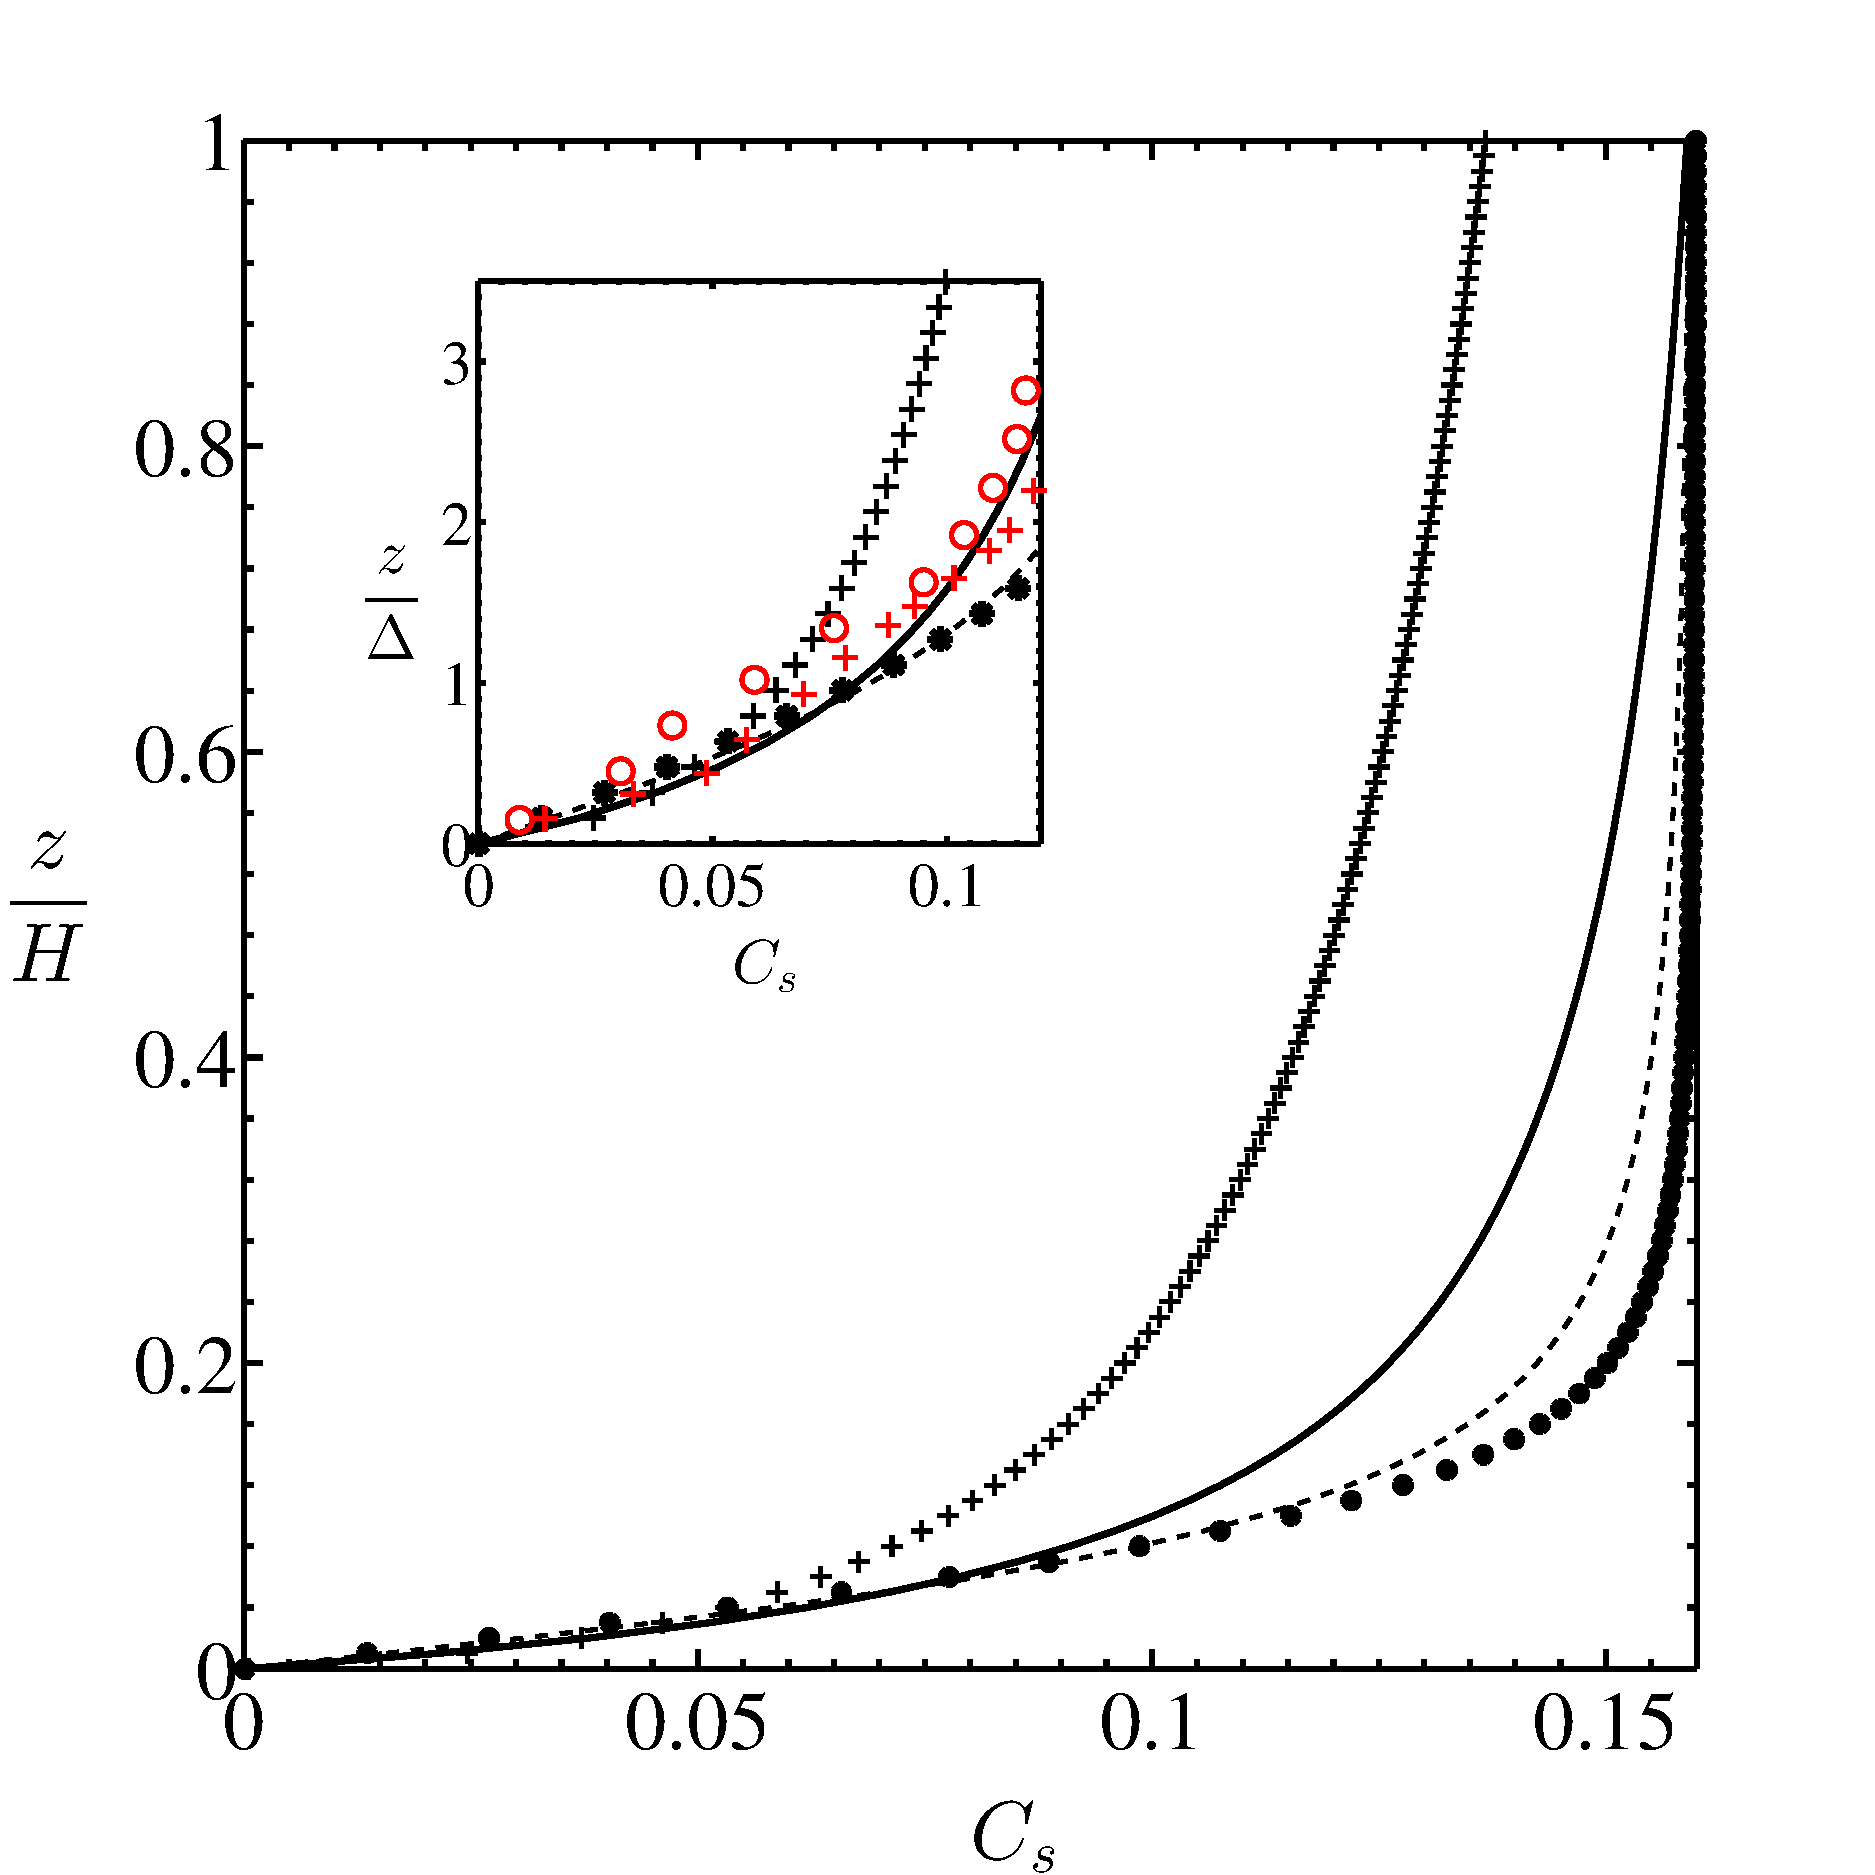
\includegraphics[width=\linewidth]{Figure/Smag2b.pdf}
                \caption{}
                \label{fig:figure_smag}
        \end{subfigure}%
        \centering
        \begin{subfigure}[t]{0.5\textwidth}
                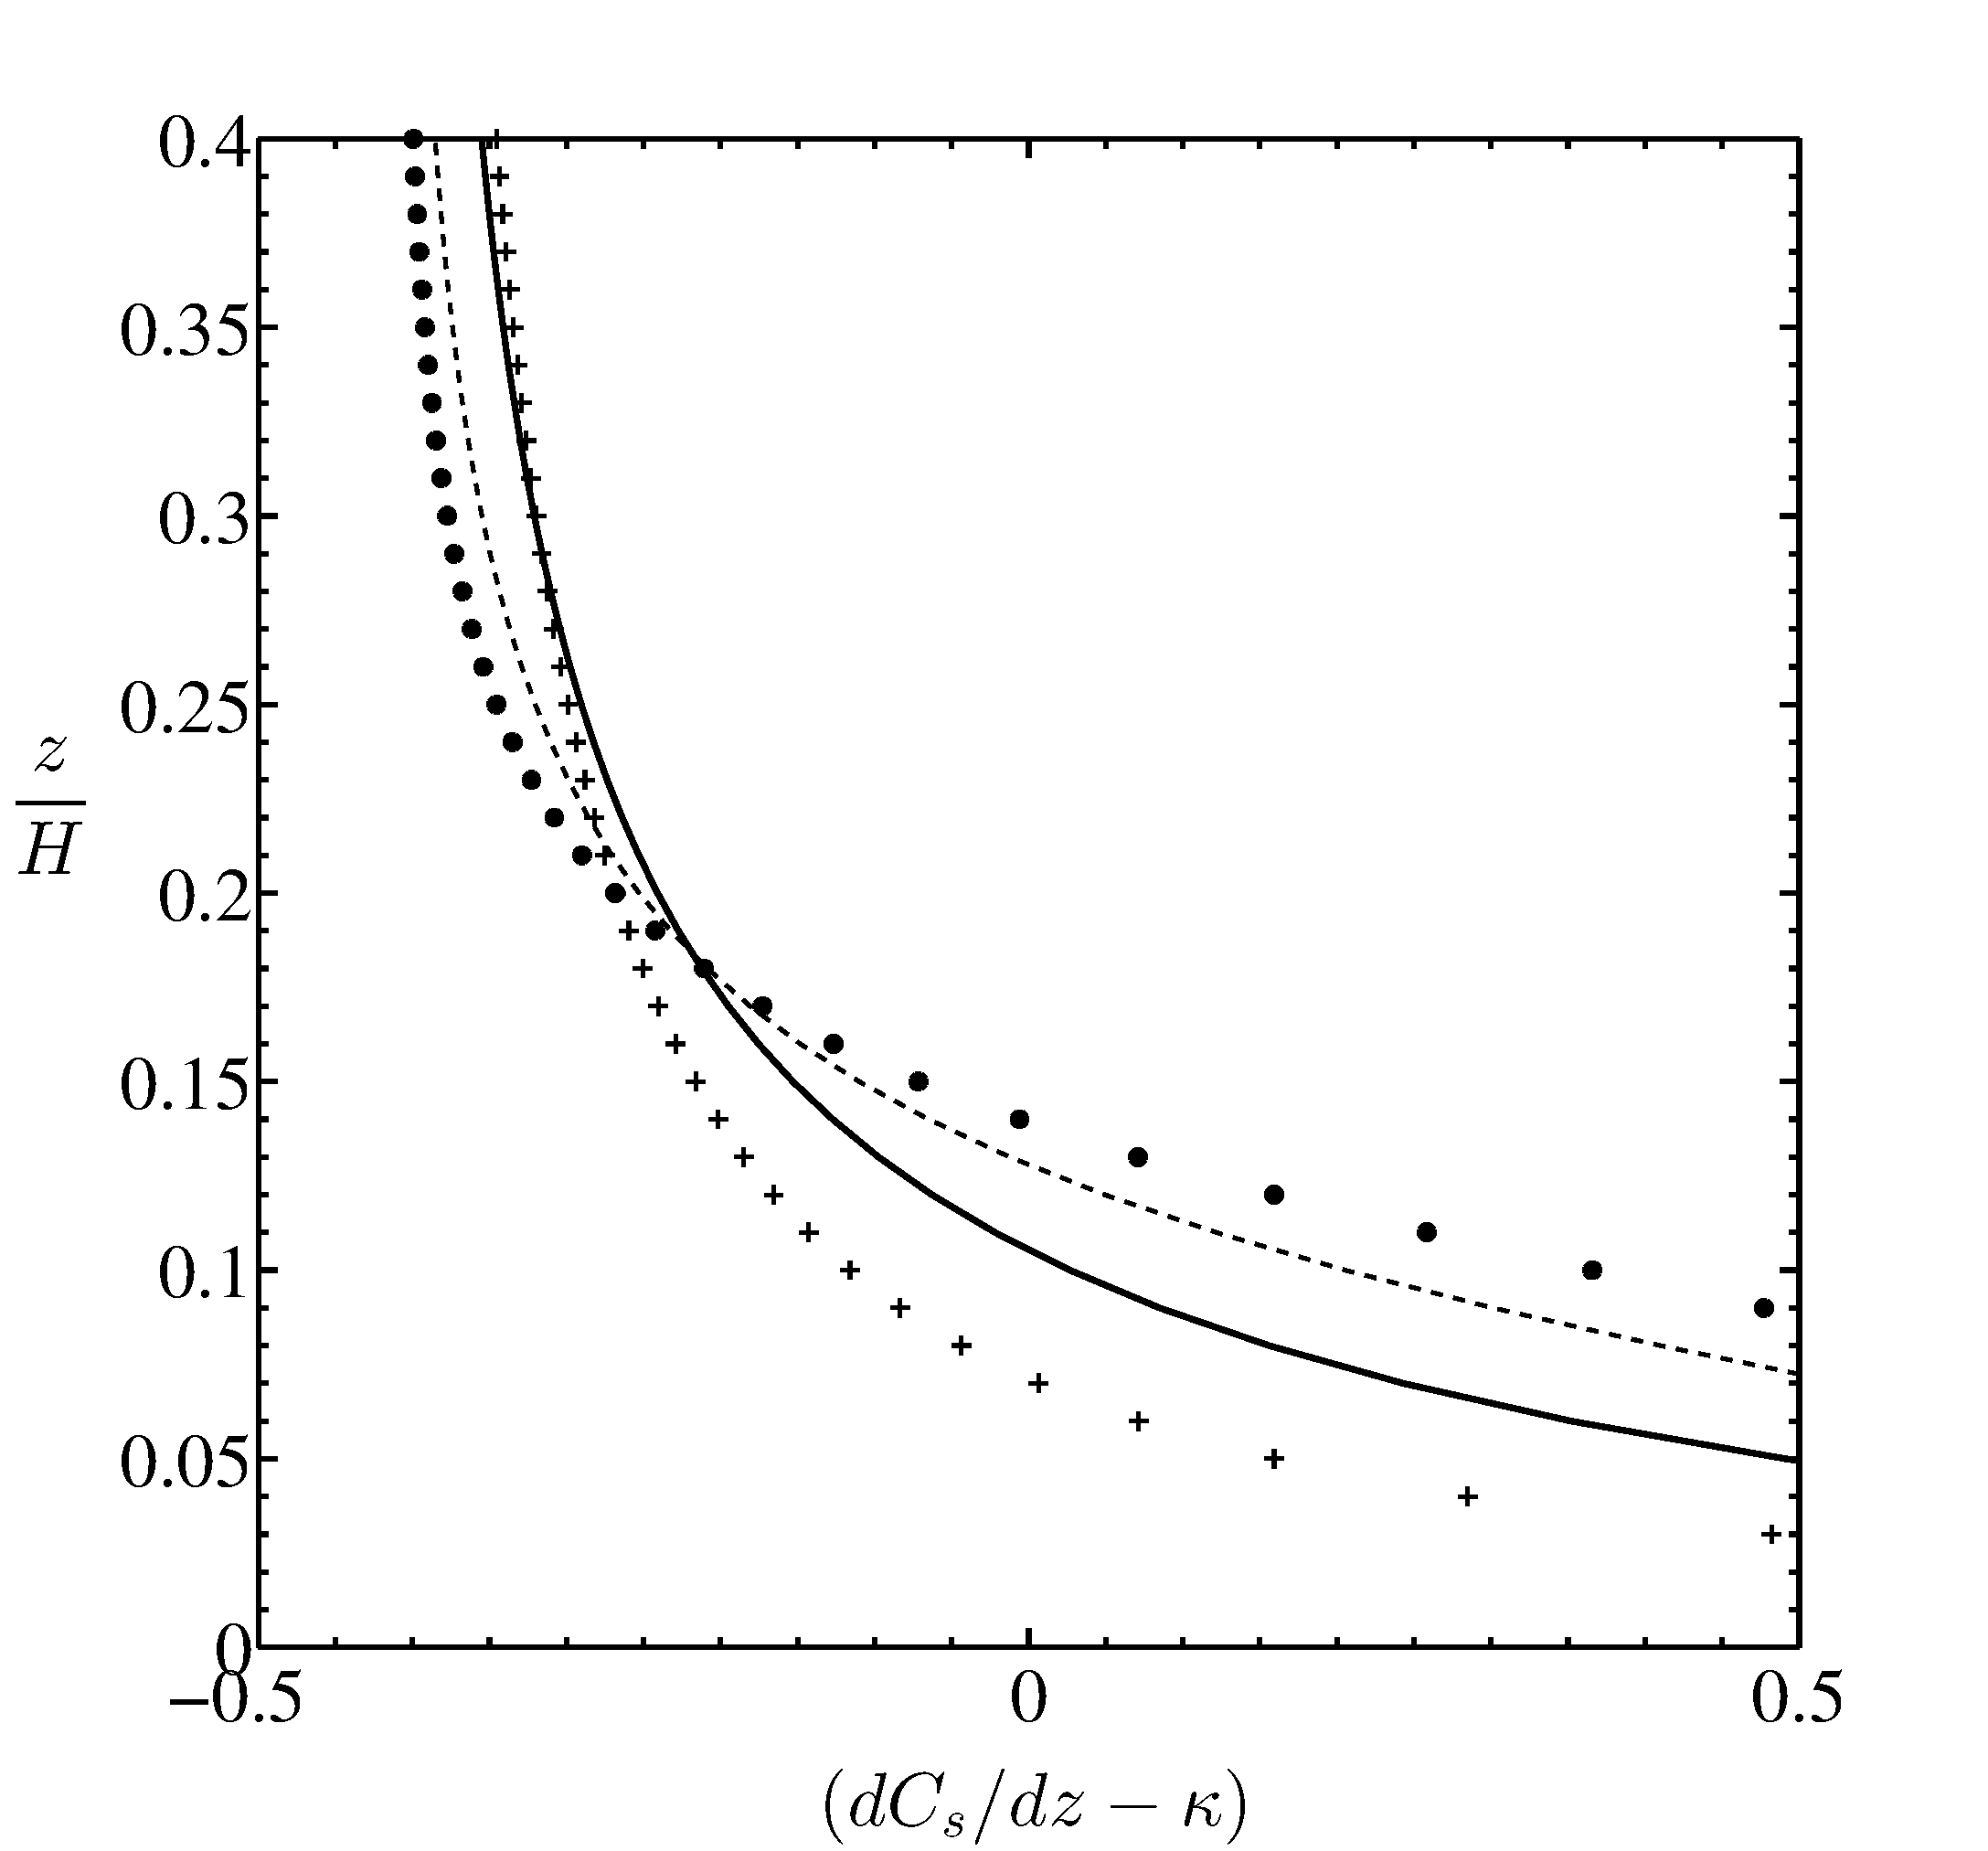
\includegraphics[width=\linewidth]{Figure/Smag2b_der.pdf}
                \caption{}
                \label{fig:smagd}
        \end{subfigure}
       \caption[Smagorinsky coefficient $C_s$ vs $z/H$ for different $(C_0, \ n)$]{(a) Smagorinsky coefficient $C_s$ vs $z/H$. Inset: variation of $C_s$ vs $z/\Delta$, zoomed-in. (b) $\frac{dC_s}{dz}-\kappa$ vs $z$.   $+$ black, $n = 0.5$; $-$ black, $n = 1$; $--$ black, $n = 2$; $\star$ black, $n = 3$; red $+$ dyn. Smagorinsky, red $o$, scale dependant dyn. Smagorinsky, Porte-Ag\'{e}l et. al (2000). $C_0 = 0.16$, fixed ($C_0 = 0.19$ for $n = 0.5$). $\kappa = 0.41$, Von Karman constant. $z_0 = 10^{-4}H$.}
\label{fig:smag}
\end{figure}

Figure~\ref{fig:figure_smag} shows the variation of Smagorinsky coefficient $C_s$ for various parameter tuples $\lbrace C_0, \ n \rbrace$ with height $z$ normalized with boundary layer thickness $H$ and also with grid scale $\Delta$. It is also observed from the  figure, that decreasing $n$ tends to smoothen the blending function in algebraic damping near wall or $\frac{dC_s}{dz}$ increases with lower value of $n$, especially in the top $10\%$ of the inner layer ($z/H \sim 0.08 - 0.10$). Additionally, with $n \downarrow$, at the upper part of ABL, the value of $C_s$ saturates to a much lower value than its classical counterpart $\sim 0.16$~\cite{lily0}.  Figure~\ref{fig:figure_smag} thus justifies the use of higher value of $C_0$ ($C_0|_{n=\frac{1}{2}} > C_0|_{n=1} > C_0|_{n=2}$), when using low value of $n$ to keep the subrid dissipation length scales ($l_f$) approximately of the same magnitudes in all the cases. It was also observed that for $n = \frac{1}{2}$, the mixing length coefficient has a reasonable comparison with the scale dependant model of Port\'{e}-Agel~\cite{porte1fun} near $z/\Delta \sim 1$.\\

In Figure~\ref{fig:smagd}, we observe that with decreasing $n$, the intersection between the curves $h(z) = (d(C_s\Delta)/dz - \kappa)$ and $g(z) = 0$ shifts downwards towards lower values of $z$ (towards log-law) within $10\%$ of the boundary layer~\cite{porte1fun,brass,meyers2} This would mean that a small region of $C_s\Delta \approx \kappa z$ can be observed within the log-layer for $n = 1/2$, which is a physically consistent phenomenon.
In this context we must mention that a relatively new methodology has already been performed to estimate the error due to SGS modelling in high Reynolds number LES done by Meyers et al.~\cite{meyers_err}. However the methodology solely concentrated on the optimization problem of the LES error metric (in wave number space) in a plane of $(C_0 \in (0.09-0.15), \ n \in(1-3))$, the two parameters in standard Smagorinsky model as suggested by Mason and Thompson~\cite{mason}. Additionally, the error metric has been compared with the log-law $\log(z/z_0)$ over the whole atmospheric boundary layer which may not be physically justifiable (see Section~\ref{nwm}). In the current study we present results with $(C_0, \ n)$ not reported previously in ABL literature~\cite{porte1fun,meyers_err,meyers2} but also elucidates a better physical understanding of the parameters $C_0, \ n$ which will be further discussed in Section~\ref{results}.
\section{Model Assumptions: Boundary conditions of ABL}\label{ablBC}
The current simulation deals with generating a feasible ABL flow field that is intercepted by the wind turbine. The simplest case is the neutral ABL simulations, where the turbulence is generated from the shear in the flow over rough wall terrain. Our present model uses $x$ as the streamwise direction, $y$ as the spanwise direction and $z$ as the wall normal direction in a cartesian framework as discussed in section~\ref{secl}. The mean streamwise velocity profile of ABL  in the surface layer (roughly $10 \sim 20\%$ of boundary layer)~\cite{basin,porte1fun,brass,meyers} can be given as
\begin{equation}
\bar{U}(z) = \frac{u_{\tau}}{\kappa}\ln \frac{z}{z_0} + \frac{u_{\tau}}{\kappa}\psi_m(\frac{z}{L_M}),\ \ \  z \gg z_0  \label{logvel}
\end{equation}
where, $u_\tau$ is the friction velocity scale, $z_0$ is the aerodynamic roughness length and $\kappa = 0.4$ is the Von Karman constant, $\psi_m$ is a non dimensional momentum stability function and $L_M$ is stability length scale by Monin and Obukhov.~\cite{obu,basin}. For neutral ABL, $L_M\rightarrow \infty$ and hence the mean velocity profile is essentially logarithmic in nature in the surface layer~\cite{obu} with $\psi_m \rightarrow 0$.\\
The boundary layer (BL) thickness for flat plate type of turbulent flows can be usually expressed as $\delta/x \sim Re_{x}^{-p}$, where $p$ is very close to 1 ($p = 0.8$ for turbulent flow over smooth flat plate)\cite{schlichting}. Consequently, the streamwise growth of the turbulent BL, could be expressed as $d\delta/dx \sim Re_{x}^{-(1+p)} $.
Since $Re_x \approx 10^8-10^{12}$ for ABL flows, the growth of the turbulent BL $d\delta/dx \approx 0$ rendering periodic boundary condition in the homogeneous streamwise direction feasible. The spanwise boundary conditions are periodic since it is consistent with the physics of the flow. The top boundary condition is a stress free lid similar to the flat plate flow, i.e., $d{\tilde{u}}_{x}/dz = d{\tilde{u}}_{y}/dz = {\tilde{u}}_{z} = 0$. For extremely high $Re$ ABL flows, the viscous sublayer $\delta_\nu/\delta \sim O(Re_{\tau}^{-1}) \approx 0$, and the aerodynamic roughness $z_0 \gg \delta_\nu$ ($\delta_{\nu} = \nu/u_{\tau}$, $\delta$ ABL thickness). Since the viscous layer cannot be resolved in such simulations, the use of shear-stress boundary conditions as near-wall modelling LES becomes imperative. Consequently, the bottom rough wall model for ABL has been developed from the log-law of the wall coupled with Monin-Obukhov similarity theory~\cite{obu} and near wall shear stress model of Schumann~\cite{schumann} and was further used by Businger et al.~\cite{basin}, Moeng ~\cite{moeng1} and Stoll and Port$\acute{e}$-Agel ~\cite{porte1a}.
\subsection{Near Wall Modelling}\label{nwm}
\par
\ \ \ We now discuss in details the complete approximate boundary conditions which we use at the bottom ``wall". For the mathematical formalism of the closure of momentum flux at bottom wall boundary condition see Appendix~\ref{stresseq}.\\
\  From now onwards, we refer to the momentum flux (shear stress) with the notation $\tau_{,s}$ for brevity. The shear stress boundary conditions for near-wall modelling are calculated from the ``in-phase" filtered resolved velocity fields half a grid node away from the ``wall" (non-local dependance)~\cite{bers} satisfying log-law (also from Monin-Obukov similarity theory)~\cite{obu} near the wall in Reynolds-average sense~\cite{pio2,jimtech,lars}. To complete the bottom wall boundary conditions we also invoke a no-penetration condition $\widetilde{w} \ = \ 0$ which is consistent with the physics of near wall large eddies~\cite{maxwell,porte1fun,bers}.
\begin{equation}
\frac{\tau_{i,zs}}{\rho} = -\kappa^{2}\frac{\widehat{\widetilde{u}}_{i,\frac{\Delta z}{2}}(x,y,t)\widehat{\widetilde{u}}_{r,\frac{\Delta z}{2}}(x,y,t)}{\log (\frac{z}{z_0})\Big \vert_{\frac{\Delta z}{2}}^{2}} \ \ \ \  \forall i = x,y \label{stress}
\end{equation}
The subscript ``s" represents shear stress at the wall surface and the ``tilde" in Equation(~\ref{stress}) represents implicit grid filtering in LES, while in SEM, the explicit filtering represented by the ``hat" is carried out in modal space by attenuating $n$ (usually 2--4) highest Legendre polynomial modes (See Appendix~\ref{elfilt} for details). The explicit filtering is done in an effort to minimize the log-layer mismatch
(overshoot of slope of logarithmic mean velocity profile observed in high $Re$ flows)~\cite{sull,bou1,chow,brass,meyers2}. 
Similar trends of incorrect slopes in logarithmic profiles has been observed by Piomelli and Ballaras~\cite{pio2} at lower Reynolds number ($Re\sim 10^6$) LES and DES (detached-eddy simulation, wall-layer RANS) which has been attributed to the artificial eddies being generated in the wall-outer layer~\cite{bag2}. This is intriguing to note, since wall-layer model also essentially considers the near wall region in the Reynolds average sense~\cite{pio2,jimtech,lars}.
\begin{equation}
\widehat{\widetilde{u}}_{r,\frac{\Delta z}{2}} = \sum_{i}\sqrt{\widehat{\widetilde{u}}_{i,\frac{\Delta z}{2}}^{2}} \ \ \ \ \ \ \ \forall i = x,y
\end{equation}
For collocated spectral element methods $\widehat{\widetilde{u}}_{i,r,\frac{\Delta z}{2}}$ are calculated as an interpolation at half wall node $\Delta z/2$ (in light of the discussion~\cite{brass,lars} ) between $\widehat{\widetilde{u}}_{\alpha}(x,y,0,t)$ and $\widehat{\widetilde{u}}_{\alpha}(x,y,z=\Delta z,t)$, $\forall \alpha = i,\ r$. Various types of interpolation has been incorporated in the present calculations involving simple mid-point ($1^{st}$ order), and exponentially accurate spectral interpolation technique, the details of which have been discussed in Section~\ref{results}. Earlier cited literature on near wall modelling~\cite{deardoff,schumann,grot,moeng1,pio_wall,bal2,porte1fun,meyers2} have generally used staggered finite-difference schemes ($2^{nd}$ to $4^{th }$ order) when using stress boundary conditions for rough wall models with $\Delta z/2$ being a physical grid distance away from the wall (since the pressure and velocity grids are different). The present paper incorporates a relatively new robust methodology for rough wall using spectral element methods~\cite{tan}, and consequently certain modifications in the conventional rough-wall models of the cited-researchers have been introduced in Equation(~\ref{stress}). It is quite fascinating to note the striking  similarity in implementation between the flux conservative finite volume/ finite difference methods, and the weak formulation of collocated SEM, where the wall model essentially is a flux-closure scheme (See Appendix~\ref{stresseq}).
The aerodynamic roughness length $z_0$ in Equation(~\ref{stress}) is a monotonic measure of physical surface roughness $h$ and their empirical relations are discussed in literature~\cite{bhag,taft,cast}. The friction velocity scale is given by $u_{\tau} = \sqrt{{\tau_{w}}/{\rho}}$, where $\tau_{w}$ is the wall shear stress, $\widetilde{F_{i}}\delta_{1i}$  is the streamwise pressure gradient that drives the ABL flow, $H$ is the depth of the boundary layer and $\rho$ is the fluid density, which can be further simplified as follows ($\overline{}$ and $\langle \ \rangle_{xy}$ are temporal and horizontal averages respectively)

\begin{equation}
\frac{\tau_{w}}{\rho} = \langle\overline{\sqrt{\tau_{x,zs}^{2} + \tau_{y,zs}^2}}\rangle_{xy} = \langle\overline{\bigg(\frac{\kappa}{\log (\frac{\Delta z}{2z_0})}\bigg)^{2}\widehat{\widetilde{u}}_{r,\frac{\Delta z}{2}}^{2}}\rangle_{xy} \sim \widetilde{F}_{1}H \sim \sqrt{\langle-\overline{\widetilde{u'}\widetilde{w'}}\rangle_{xy}} \label{stress2}
\end{equation}
Equation~\ref{stress2} provides a measure of computing $u_{\tau}$ in the calculation and all of three methods are seen to generate consistent values.
It is important to note, that the logarithmic trend of velocity profile is only justified with its mean, even though ABL community using LES framework~\cite{sull,brass,porte1a,meyers2} has used instantaneous or quasi instantaneous  (filtered) velocities in the wall model as is in the current simulation.

\section{Model Assumptions: Boundary conditions of Wind turbine Array}\label{wtBC}
The boundary conditions for the rectangular domain of wind turbine array are very similar to the ABL domain (spanwise periodic, symmetry at the top and shear stress at the bottom ``wall"), except for the streamwise direction where we choose to use a realistic inflow-outflow condition. The inflow condition is turbulent in nature and to maintain a realistic spatio-temporal coherence the inlow is being fed from a seperate precursor ABL simulation. The choice of outflow boundary conditions in our spectral element code requires a careful analysis. Invoking Equation~\ref{outflow_1} (See Appendix~\ref{out} for more mathematical details) we see that the  simplest choice of natural ``do nothing" boundary condition at the outflow would be 
\begin{equation}
(-p + \frac{1}{Re}\nabla \cdot \mathbf{u})\cdot \mathbf{n} = 0 \ \ \mbox{on} \ \ \Gamma \label{nbc1}
\end{equation}
However implementing such boundary conditions at high Reynolds number triggers amplification of outgoing large eddy structures at the outflow resulting in reflection and instability. To circumvent this problem we have used sponging by extending the domain with coarse elements and adding sufficient amount of artificial viscosity near the outflow region ensuring required dampening of the eddies before they go to the outflow boundary. However, sudden change in viscosity in the interface of physical and extended domain can be dangerous giving rise to spurious reflective waves which can potentially trigger instability. Consequently, we have extended the idea of carefully-designed non reflective sponging layer using simple Smagorinsky type viscosity in the sponge layer which restricts the indiscriminate growth of viscosity in that region. In the sponge-layer, $\nu = \nu_m + \nu_{sl}$, with $\nu_m$ being the molecular viscosity where $\nu_{sl} = (C_{sl}\Delta)^2|\widetilde{S}|$, with $ |\widetilde{S}| = \sqrt{2\widetilde{S}_{ij}\widetilde{S}_{ij}}$. $\Delta$ is metric of grid spacing scale which is similar to that in LES Smagorinsky model~\cite{smagorinsky}. In our spectral element model $C_{sl}$ is designed to grow quadratically in the form $C_{sl} = b(x-x_0)^2$, with $b = 0.25$ and $x_0$ is the end of the streamwise extent of physical domain. The natural boundary condition with a non-reflective sponge layer is seen to stabilize eddies at the outflow. Additionally, we also plan to present the results from stabilized natural boundary conditions by Dong et. al~\cite{dong} which can be given as
\begin{equation}
\boxed{-p\cdot \mathbf{n} + \frac{1}{Re}\nabla  \mathbf{u} \cdot \mathbf{n} - \frac{1}{2}\vert \mathbf{u} \vert ^{2}\Theta (\mathbf{n},\mathbf{u}) = 0 \ \ \mbox{on} \ \ \Gamma} \label{nbc2}
\end{equation}
where
$$ \Theta (\mathbf{n},\mathbf{u}) = \left(1 - \frac{\tanh(\mathbf{n} \cdot \mathbf{u})}{U\delta}\right)$$ is smooth Heaviside step function to remove sudden discontinuity of the outflow fluxes with $U, \ \delta$ being some chosen velocity and length scale in the flow and $\mathbf{n}$ is the unit normal vector at the outflow boundary. This boundary condition has been tested to stabilize energy of the system $1/2 \vert\vert \mathbf{u}\vert \vert^{2}_{L_2({\Omega})}$ (projecting NS equation with $\mathbf{u}$) compared to a simple natural boundary condition~\cite{erik} (See Equation~\ref{nbc1}).
\section{Actuator Line Model: Wind turbine}
Actuator line model was first developed by S{\o}rensen \& Shen~\cite{sorensen:02} and Troldborg~\cite{troldborg}, later used by Churchfield et al.~\cite{churchfield,churchfield_2} in finite volume computations and was extended to the current spectral element code by Peet et al.~\cite{peet2}. The idea of the actuator line model is that the influence of the rotating blades is modelled as a sum of discrete body forces introduced into the flow field. Thus, resolving boundary layer around the blades can be avoided, and simple rectilinear grid can be used.  In an actuator line model, the blades are divided into the elements, similar to BEM, and the local lift ($L$) and drag ($D$) force experienced by each element is calculated as
\begin{equation}
L=\frac{1}{2}C_l(\alpha)\,\rho\,V_{rel}^2\,c\,w,
\end{equation}
\begin{equation}
D=\frac{1}{2}C_d(\alpha)\,\rho\,V_{rel}^2\,c\,w,
\end{equation}
where $C_l(\alpha)$ and $C_d(\alpha)$ are the lift and drag coefficients respectively, $\alpha$ is the local angle of attack, $\rho$ is the fluid density, $V_{rel}$ is the local velocity magnitude relative to the rotating blade, $c$ is the local chord length, and $w$ is the actuator element width. Considering velocity triangles for the rotating blade,~\cite{sorensen:02, troldborg} as shown in Figure~\ref{f:triangle} the local relative velocity magnitude $V_{rel}$ can be given as
\begin{equation}
V_{rel}=\sqrt{V^2_x+(\Omega\,r-V_{\theta})^2},
\end{equation}
where, $\Omega$ is the rotor rotational speed, $V_x$ and $V_{\theta}$ are the velocity components in the axial direction $x$ (perpendicular to the plane of rotation), and in circumferential direction (in the plane of rotation corresponding to $y z$ plane) respectively, $r$ is the radial coordinate of the actuator element. Local angle of attack $\alpha$ is computed as $\alpha=\phi-\gamma$, where $\phi$ is the angle between the relative velocity $V_{rel}$ and the rotor plane
\begin{equation}
\phi=\tan^{-1}\big(\frac{V_x}{\Omega\,r-V_\theta} \big)
\end{equation}
and $\gamma$ is the local pitch angle. The element lift and drag coefficients $C_l(\alpha)$, $C_d(\alpha)$ as function of $\alpha$ can be determined from the lookup tables.
\begin{figure}
\centering
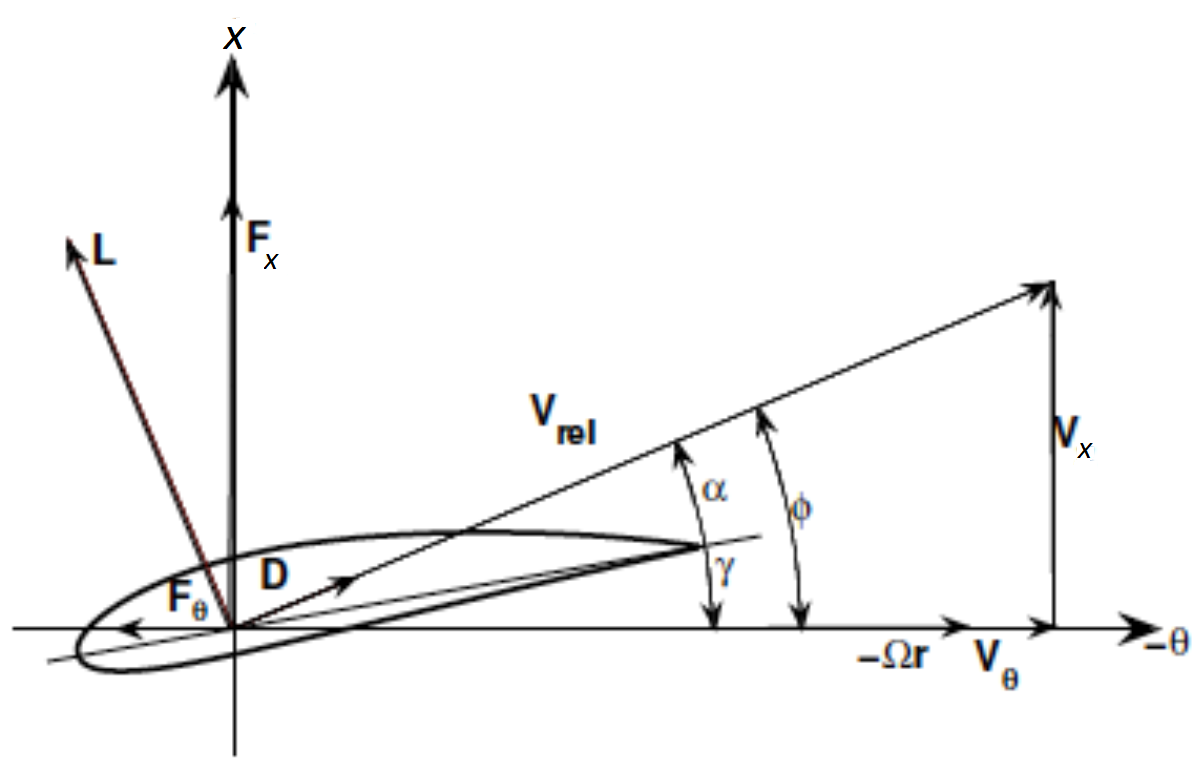
\includegraphics[width=0.45\textwidth]{Figure/triangle.png}\\
 \caption[Velocity triangle on a wind turbine blade]{Velocity triangle for the determination of the local relative velocity on a turbine blade.}
 \label{f:triangle}
\end{figure}
After calculating the local aerodynamic force $\vec{f}= L\vec{e_L}+D\vec{e_D}$, its influence, $-\vec{f}$, on the flow is incorporated as a sum of discrete forces (here $\vec{e_L}$ and $\vec{e_D}$ are the unit vectors in the direction of the local lift and drag, respectively). The total force from all the blade elements experienced by the fluid is given by
\begin{equation}
\vec{F}(x,\,y,\,z,\,t)=-\sum_{i=1}^{N}\vec{f}(x_i,\,y_i,\,z_i,\,t)\,\delta(|\vec {r}-\vec{r_i}|) \label{force}
\end{equation}
where, $\delta(|\vec {r}-\vec{r_i}|)$ is the Dirac delta function. Equation(\ref{force}) represents the discrete force model in a continuous form by using delta function. To avoid  singularities, the forces are distributed smoothly on several mesh points by using the Gaussian weight function (smeared out delta function),
\begin{equation}
\eta_{\,\epsilon}(d)=\frac{1}{\epsilon^3\pi^{3/2}}\exp\big[-\big(\frac{d}{\epsilon}\big)^2\big],
\end{equation}
with the modified force term as
\begin{equation}
\vec{F}(x,\,y,\,z,\,t)=-\sum_{i=1}^{N}\vec{f}(x_i,\,y_i,\,z_i,\,t)\,\eta_{\,\epsilon}(|\vec {r}-\vec{r_i}|),
\end{equation}
where the summation is over all $N$ blade elements, $x_i,y_i,z_i$ are the local coordinates of each blade element, and $|\vec {r}-\vec{r_i}|$ is the distance between the current point in the flow and the center of the blade element. Several studies have been carried out for the choice of an optimal Gaussian width $\epsilon$~\cite{troldborg, martinez}. The value of $\epsilon=2\,w$ proposed by Troldborg~\cite{troldborg} is used in the current study.




